\documentclass[11pt]{extarticle}
\usepackage{mathtools}
\usepackage[a4paper, total={6in, 8.5in}]{geometry}
\usepackage{graphicx}
\usepackage{subfig}
\usepackage{amssymb}
\usepackage{amsmath}
\usepackage{pythonhighlight}
\usepackage{pdfpages}
\usepackage[T1]{fontenc}
\usepackage[utf8]{inputenc}
\usepackage{fancyhdr}
\usepackage{pythonhighlight}
\usepackage{changepage}
\usepackage{slashbox}
\usepackage{floatrow}
\usepackage{subfig}
\usepackage{listings}
\usepackage[hidelinks]{hyperref}
\usepackage{fontawesome}
\usepackage{color} %red, green, blue, yellow, cyan, magenta, black, white
\definecolor{mygreen}{RGB}{28,172,0} % color values Red, Green, Blue
\definecolor{mylilas}{RGB}{170,55,241}


\floatsetup[table]{capposition=top}

\sloppy
\definecolor{lightgray}{gray}{0.5}
\setlength{\parindent}{0pt}
\setlength{\headheight}{14pt}

\renewcommand{\headrulewidth}{.4mm} % header line width
\newcommand{\norm}[1]{\left\lVert#1\right\rVert}


\pagestyle{fancy}
\fancyhf{}
\fancyhfoffset[L]{-1cm} % left extra length
\fancyhfoffset[R]{-1cm} % right extra length
\rhead{\bfseries Kutay U\u{g}urlu 2232841}
\lhead{EE583 Homework 2}
\rfoot{}

\DeclarePairedDelimiter\ceil{\lceil}{\rceil}
\DeclarePairedDelimiter\floor{\lfloor}{\rfloor}

\author{Kutay U\u{g}urlu 2232841}

\begin{document}

\lstset{language=Matlab,%
    %basicstyle=\color{red},
    breaklines=true,%
    morekeywords={matlab2tikz},
    keywordstyle=\color{blue},%
    morekeywords=[2]{1}, keywordstyle=[2]{\color{black}},
    identifierstyle=\color{black},%
    stringstyle=\color{mylilas},
    commentstyle=\color{mygreen},%
    showstringspaces=false,%without this there will be a symbol in the places where there is a space
    numbers=left,%
    numberstyle={\tiny \color{black}},% size of the numbers
    numbersep=9pt, % this defines how far the numbers are from the text
    emph=[1]{for,end,break},emphstyle=[1]\color{red}, %some words to emphasise
    %emph=[2]{word1,word2}, emphstyle=[2]{style},    
}

\fancyfoot[C]{\thepage}
\title{\LARGE \LARGE EE583 Pattern Recognition HW2}

\maketitle{\LARGE}

\pagebreak


\section{Question 1}

Maximum Likelihood Estimate of Multivariate Gaussian random variable are calculated as:
\begin{itemize}
    \item $\hat{\mu} = \frac{1}{m}\sum_{i=1}^mX^{(i)}$
    \item $\hat{\Sigma} = \frac{1}{m}\sum_{i=1}^m(X^{(i)}-\hat{\mu})(X^{(i)}-\hat{\mu})^T$
\end{itemize}
where $X^{(i)}$ is the $i^{th}$ observation.\\

The given MATLAB code in Section \ref{subsec:Q1_code} produces the following results:\\
\begin{minipage}{0.2\textwidth}
    $m = 10$
\end{minipage}
\begin{minipage}{0.35\textwidth}
    $\hat{\mu} = \begin{bmatrix} -0.4519 & 1.0984 \end{bmatrix}$
\end{minipage}
\begin{minipage}{0.66\textwidth}
    $\hat{\Sigma} = \begin{bmatrix} 0.3191 & 0.1799 \\ 0.1799 & 0.6506 \end{bmatrix}$
\end{minipage}
\begin{minipage}{0.2\textwidth}
    $m = 1000$
\end{minipage}
\begin{minipage}{0.35\textwidth}
    $\hat{\mu} = \begin{bmatrix} -0.7367 & 0.5176 \end{bmatrix}$
\end{minipage}
\begin{minipage}{0.66\textwidth}
    $\hat{\Sigma} = \begin{bmatrix} 0.4730 & 0.2925 \\ 0.2925 & 0.8079 \end{bmatrix}$
\end{minipage}
It is observed that the estimations get more accurate, \textit{i.e.} the calculated metrics get closer to the original ones,  with increasing number of samples.

\section{Question 2}

The ML estimate is calculated using mean of the generated data. On the other hand, to calculate the MAP estimate of $\mu$, following formula is utilized:\\

\begin{equation}
    \label{eq:mu_map}
    {\hat{\mu}}_{n} = \frac{n{\sigma_0}^2}{n{\sigma_0}^2+\sigma^2} \frac{1}{n}\sum_{i=1}^n x_i + \frac{{\sigma}^2\mu_0}{n{\sigma_0}^2+\sigma^2}
\end{equation}

The formula given is a normalized weighted average of mean of the training data and mean assumed previously.
The mean estimate in Eq. \ref{eq:mu_map} converges to sample mean when $n \rightarrow \infty$. For $n=0$, the
estimate is just the prior mean, and it gets closer to the sample mean when n increases. Therefore, one would expect to see an
estimate around $\mu_0$ for "small" n. However,
even for small values of n, such as 25, the weight of the sample mean approaches to 0.95.  Still, for small n,
the sample mean does not converge to the actual sample mean, and in one experiment, I have made the following observations.

\subsection{25 Samples}
\begin{minipage}{0.3\textwidth}
    ${\hat{x}}_{ML} = 2.8995$
\end{minipage}
\begin{minipage}{0.6\textwidth}
    ${\hat{x}}_{MAP} = 2.9019$
\end{minipage}

\subsection{1000 samples}
\begin{minipage}{0.3\textwidth}
    ${\hat{x}}_{ML} = 2.9983$
\end{minipage}
\begin{minipage}{0.6\textwidth}
    ${\hat{x}}_{MAP} = 2.9984$
\end{minipage}
\vspace*{0.5cm}

With increasing n, the sample mean dominates the estimate for sure.
But for small n around 20, the estimate is highly dependent on the sample mean.
It is also observed that, the estimates gets closer with increasing number of training samples.

\section{Question 3}
\begin{center}
    \begin{figure}[h]
        \begin{tabular}{cc}
            \subfloat[Training and Test data]{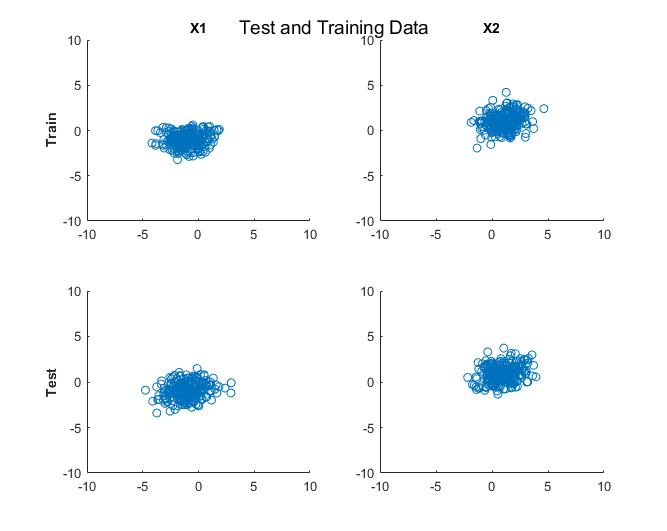
\includegraphics[width = 2.5in]{q3foursfinal.png}} &
            \subfloat[Decision Boundaries and Error Rates]{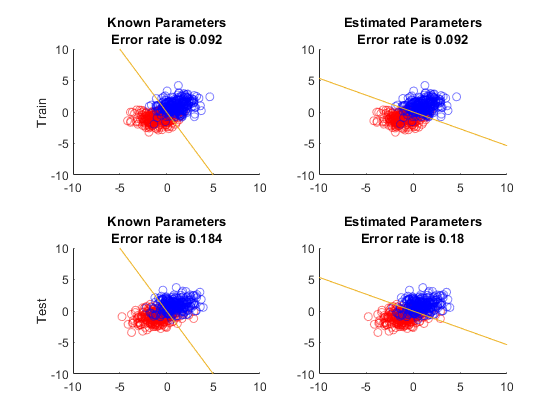
\includegraphics[width = 2.5in]{q3decfinal.png}} \\
        \end{tabular}
        \caption{Data distributions and Decision Boundaries}
        \label{fig:q3fig}
    \end{figure}
\end{center}
As expected, training accuracy is higher than the test accuracy. Furthermore, decision boundaries obtained with estimated parameters
resulted in lower accuracy, since the minimum error rate classifier boundaries are calculated analytically with already known distribution parameters.

\section{Question 4}
\begin{center}
    \begin{figure}[h]
        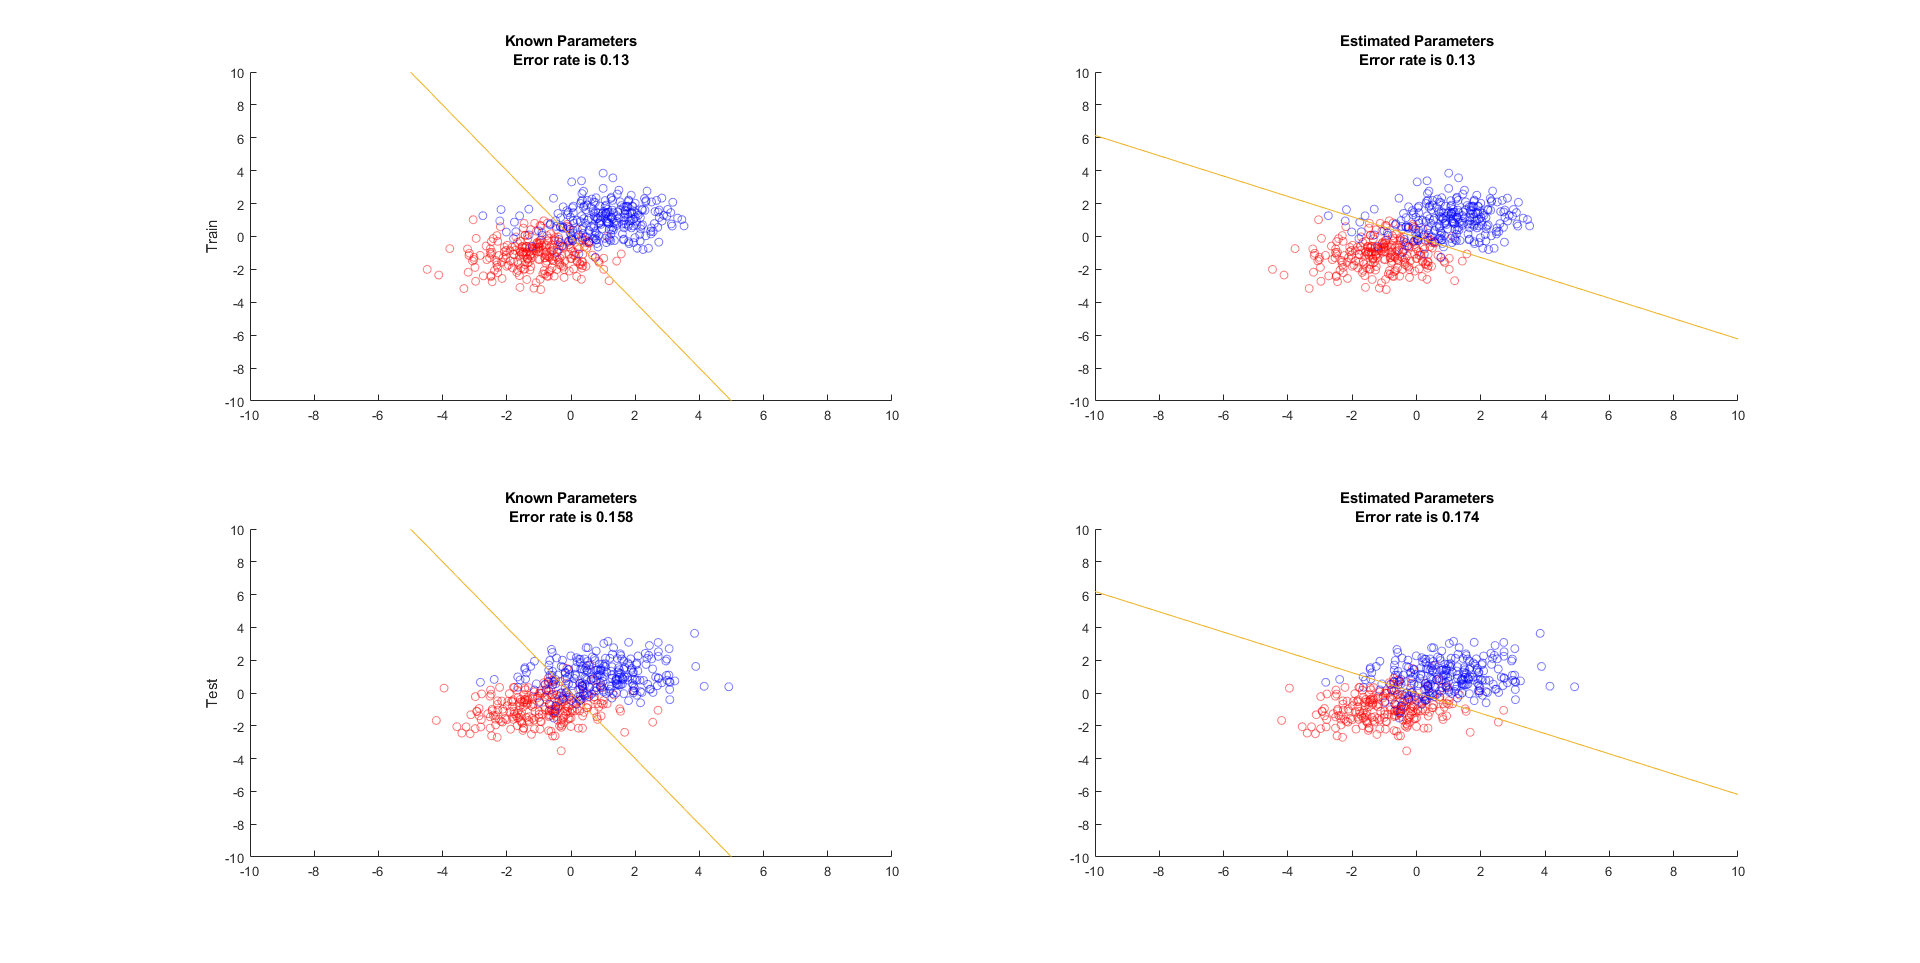
\includegraphics[width = 5in,height=6cm]{Q4.png}
        \caption{Parzen window estimation results}
        \label{fig:parzen}
    \end{figure}
\end{center}
The selection of initial volume and volume shrinking formula are presented in subsection \ref{subsec:Q4_code}.

\section{Question 5}
\begin{center}
    \begin{figure}[h]
        \begin{tabular}{cc}
            \subfloat[PCA Projection onto 1D]{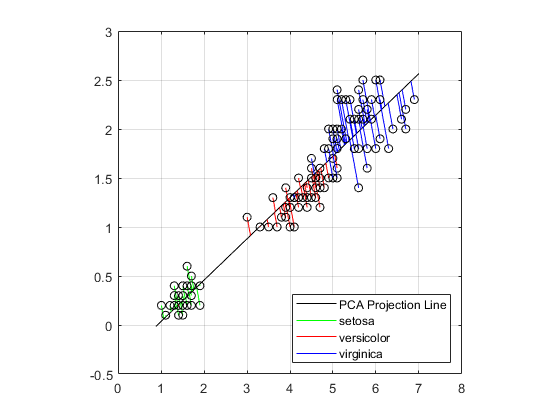
\includegraphics[width = 2.5in]{Q5project.png}} &
            \subfloat[Histograms]{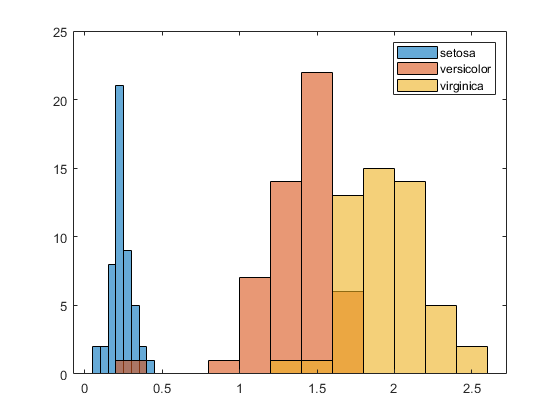
\includegraphics[width = 2.5in]{Q5hist.png}}                  \\
        \end{tabular}
        \caption{PCA Projection and histogram}
        \label{fig:q5fig}
    \end{figure}
\end{center}

\pagebreak
\section{APPENDIX}
The code given in this section is shared \href{https://github.com/kutay-ugurlu/Pattern-Recognition/tree/master/HW2}{@\faGithubSquare}.
\subsection{Q1}\label{subsec:Q1_code}
\lstinputlisting{HW2_Q1.m}
\pagebreak
\subsection{Q2} \label{subsec:Q2_code}
\lstinputlisting{HW2_Q2.m}
\pagebreak
\subsection{Q3}\label{subsec:Q3_code}
\lstinputlisting{HW2_Q3.m}
\pagebreak
\subsection{Q4}\label{subsec:Q4_code}
\lstinputlisting{HW2_Q4.m}
\pagebreak
\subsection{Q5}\label{subsec:Q5_code}
\lstinputlisting{HW2_Q5.m}
\end{document}